\documentclass[nooutcomes]{ximera}
%\documentclass[space,handout,nooutcomes]{ximera}

% For preamble materials

\usepackage{pgf,tikz}
\usepackage{mathrsfs}
\usetikzlibrary{arrows}
\usepackage{framed}
\usepackage{amsmath}
\pgfplotsset{compat=1.17}

\def\fixnote#1{\begin{framed}{\textcolor{red}{Fix note: #1}}\end{framed}}  % Allows insertion of red notes about needed edits
%\def\fixnote#1{}

\def\detail#1{{\textcolor{blue}{Detail: #1}}}   

\pdfOnly{\renewenvironment{image}[1][]{\begin{center}}{\end{center}}}

\graphicspath{
  {./}
  {chapter1/}
  {chapter2/}
  {chapter4/}
  {proofs/}
  {graphics/}
  {../graphics/}
}

\newenvironment{sectionOutcomes}{}{}


%%% This set of code is all of our user defined commands
\newcommand{\bysame}{\mbox{\rule{3em}{.4pt}}\,}
\newcommand{\N}{\mathbb N}
\newcommand{\C}{\mathbb C}
\newcommand{\W}{\mathbb W}
\newcommand{\Z}{\mathbb Z}
\newcommand{\Q}{\mathbb Q}
\newcommand{\R}{\mathbb R}
\newcommand{\A}{\mathbb A}
\newcommand{\D}{\mathcal D}
\newcommand{\F}{\mathcal F}
\newcommand{\ph}{\varphi}
\newcommand{\ep}{\varepsilon}
\newcommand{\aph}{\alpha}
\newcommand{\QM}{\begin{center}{\huge\textbf{?}}\end{center}}

\renewcommand{\le}{\leqslant}
\renewcommand{\ge}{\geqslant}
\renewcommand{\a}{\wedge}
\renewcommand{\v}{\vee}
\renewcommand{\l}{\ell}
\newcommand{\mat}{\mathsf}
\renewcommand{\vec}{\mathbf}
\renewcommand{\subset}{\subseteq}
\renewcommand{\supset}{\supseteq}
%\renewcommand{\emptyset}{\varnothing}
%\newcommand{\xto}{\xrightarrow}
%\renewcommand{\qedsymbol}{$\blacksquare$}
%\newcommand{\bibname}{References and Further Reading}
%\renewcommand{\bar}{\protect\overline}
%\renewcommand{\hat}{\protect\widehat}
%\renewcommand{\tilde}{\widetilde}
%\newcommand{\tri}{\triangle}
%\newcommand{\minipad}{\vspace{1ex}}
%\newcommand{\leftexp}[2]{{\vphantom{#2}}^{#1}{#2}}

%% More user defined commands
\renewcommand{\epsilon}{\varepsilon}
\renewcommand{\theta}{\vartheta} %% only for kmath
\renewcommand{\l}{\ell}
\renewcommand{\d}{\, d}
\newcommand{\ddx}{\frac{d}{dx}}
\newcommand{\dydx}{\frac{dy}{dx}}


\usepackage{bigstrut}


\title{Proof by Picture}
\author{Bart Snapp and Brad Findell}
\begin{document}
\begin{abstract}
Short-answer proofs by pictures. 
\end{abstract}
\maketitle


\begin{problem}
Explain how the following picture ``proves'' that
  the area of a right triangle is half the base times the height.
\begin{image}
\definecolor{qqwuqq}{rgb}{0.,0.392,0.}
\begin{tikzpicture}[line cap=round,line join=round,>=triangle 45,x=1.0cm,y=1.0cm]
\clip(-0.1,-0.1) rectangle (4.1,3.1);
\draw[line width=0.8pt,color=qqwuqq,fill=qqwuqq,fill opacity=0.10] (0.28,0.) -- (0.28,0.28) -- (0.,0.28) -- (0.,0.) -- cycle; 
\draw [line width=0.8pt] (0.,3.)-- (0.,0.);
\draw [line width=0.8pt] (0.,0.)-- (4.,0.);
\draw [line width=0.8pt] (4.,0.)-- (0.,3.);
\draw [line width=0.8pt,dash pattern=on 2pt off 2pt] (0.,3.)-- (4.,3.);
\draw [line width=0.8pt,dash pattern=on 2pt off 2pt] (4.,3.)-- (4.,0.);
\end{tikzpicture}
%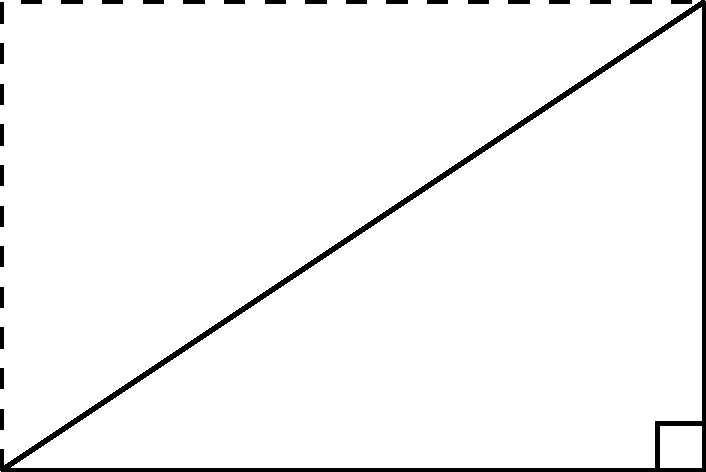
\includegraphics{pbpAreaRight.png}
\end{image}
\begin{freeResponse}
\begin{hint}
The area of the rectangle is base times height.  The rectangle is made up of two congruent right triangles.  Because congruent triangles have the same area, the area of each right triangle is \wordChoice{\choice{equal to}\choice[correct]{half}\choice{double}} the area of the rectangle.  
\end{hint}
\end{freeResponse}
\end{problem}

\begin{problem}
Suppose you know that the area of a \textbf{right} triangle is
  half the base times the height. Explain how the following picture
  ``proves'' that the area of \textbf{every} triangle is half the base times the
  height.
\begin{image}
\definecolor{qqwuqq}{rgb}{0.,0.392,0.}
\begin{tikzpicture}[scale=0.8,line cap=round,line join=round,>=triangle 45,x=1.0cm,y=1.0cm]
\clip(-0.5,-0.05) rectangle (5,2.55);
\draw[line width=0.8pt,color=qqwuqq,fill=qqwuqq,fill opacity=0.1] (3.,0.1954) -- (2.8046,0.1954) -- (2.8046,0.) -- (3.,0.) -- cycle; 
\draw[line width=0.8pt,color=qqwuqq,fill=qqwuqq,fill opacity=0.1] (3.1954,0.) -- (3.1954,0.1954) -- (3.,0.1954) -- (3.,0.) -- cycle; 
\draw [line width=0.8pt] (0.,0.)-- (3.,2.5);
\draw [line width=0.8pt] (3.,2.5)-- (4.,0.);
\draw [line width=0.8pt] (4.,0.)-- (0.,0.);
\draw [line width=0.8pt] (0.,0.)-- (3.,0.);
\draw [line width=0.8pt] (3.,0.)-- (4.,0.);
\draw [line width=0.8pt,dash pattern=on 2pt off 2pt] (3.,0.)-- (3.,2.5);
\end{tikzpicture}
%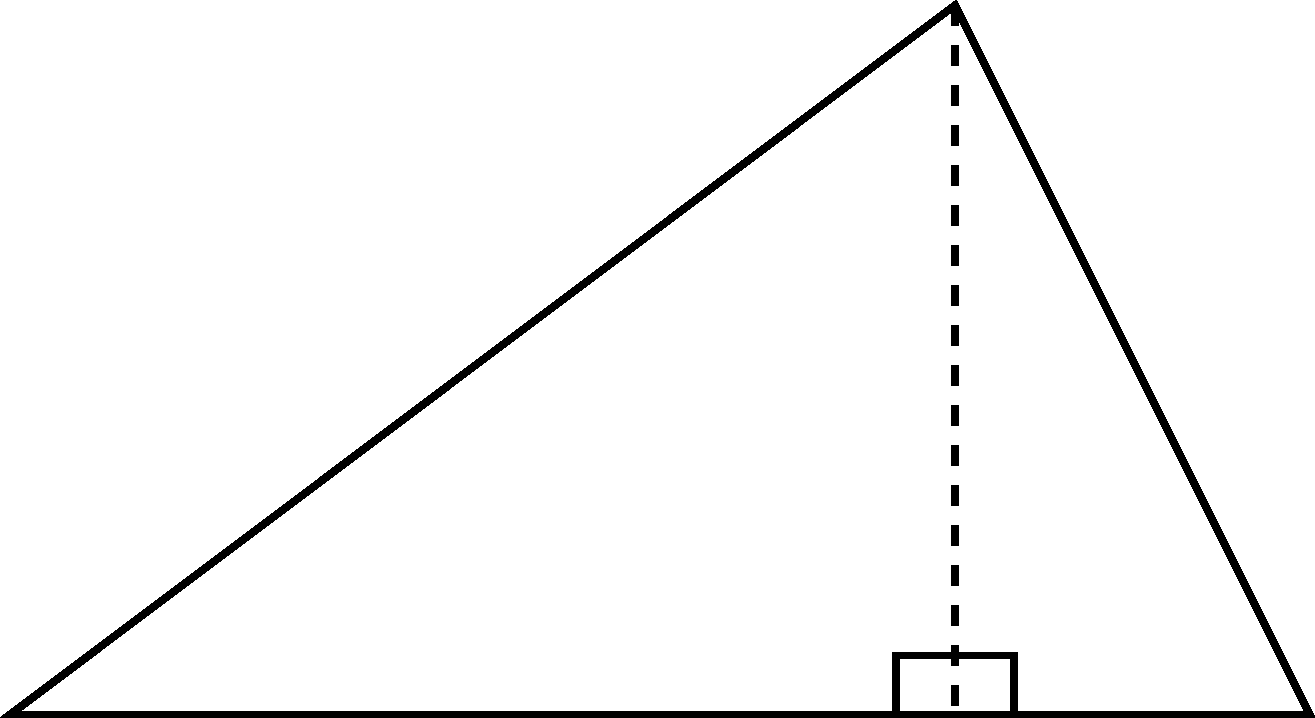
\includegraphics{pbpDisTri.png}
\end{image}

\begin{freeResponse}
\begin{hint}
The whole triangle is made up of two right triangles.  Call the bases of the small right triangles $b_1$ and $b_2$, and call the base of the large (combined) triangle $b$.  Then $b=b_1+b_2$, and the three triangles all have the same height, $h$.   The area of the whole triangle is the sum of the areas of the two right triangles:  
\[
\mathrm{area} =  \frac{hb_1}{2}+ \frac{hb_2}{2}= \frac{h(b_1 + b_2)}{2} = \answer{bh/2}
\]
because $b=b_1+b_2$.
\end{hint}
\end{freeResponse}
\end{problem}

\begin{problem}
Now suppose that a student, say \textit{Geometry Giorgio} attempts to
solve a similar problem. Again knowing that the area of a right
triangle is half the base times the height, he draws the following
picture:
\begin{image}
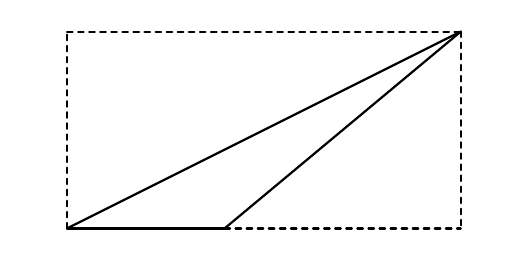
\begin{tikzpicture}[line cap=round,line join=round,>=triangle 45,x=1.0cm,y=1.0cm]
\clip(-0.5,-0.05) rectangle (5.25,2.55);
\draw [line width=0.8pt,dash pattern=on 2pt off 2pt] (0.,0.)-- (0.,2.5);
\draw [line width=0.8pt,dash pattern=on 2pt off 2pt] (0.,2.5)-- (5.,2.5);
\draw [line width=0.8pt,dash pattern=on 2pt off 2pt] (5.,2.5)-- (5.,0.);
\draw [line width=0.8pt] (5.,2.5)-- (2.,0.);
\draw [line width=0.8pt] (5.,2.5)-- (0.,0.);
\draw [line width=0.8pt] (0.,0.)-- (2.,0.);
\draw [line width=0.8pt,dash pattern=on 2pt off 2pt] (2.,0.)-- (5.,0.);
\end{tikzpicture}
%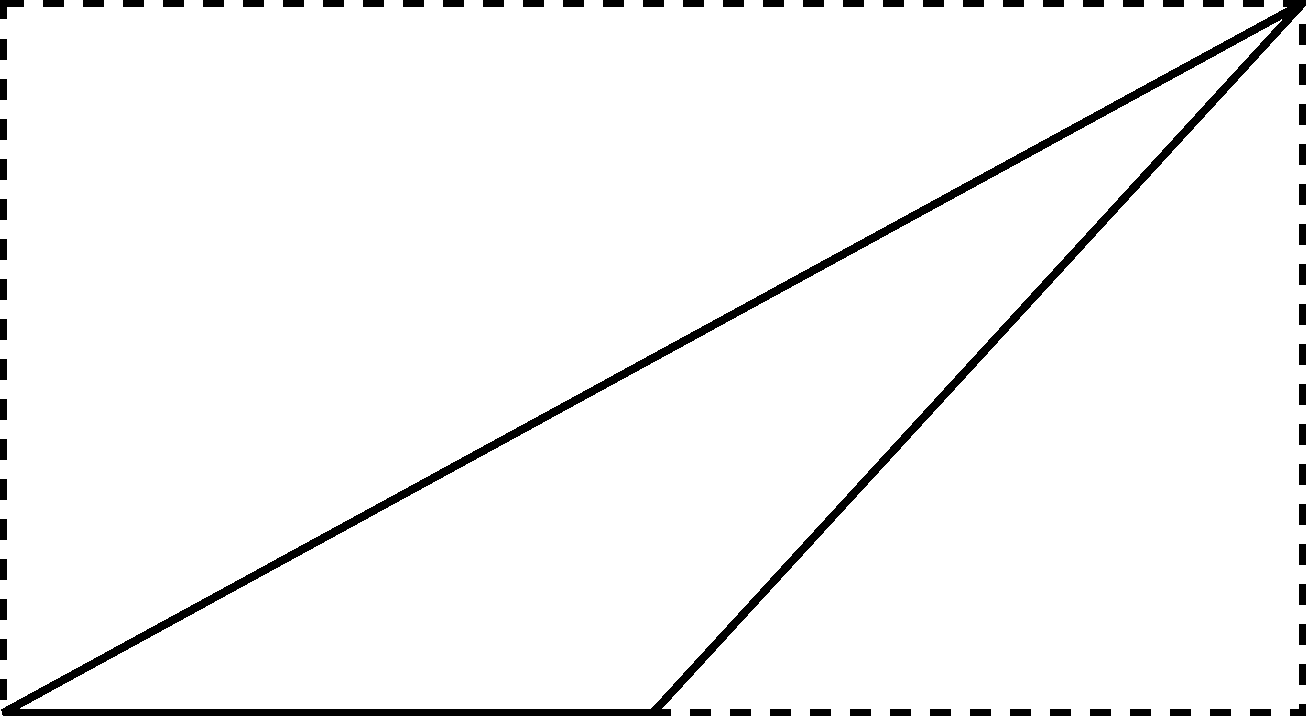
\includegraphics{pbpDisTriGio.png}
\end{image}
\textit{Geometry Giorgio} states that the diagonal line cuts the
rectangle in half, and thus the area of the triangle is half the base
times the height. Is this correct reasoning? If so, give a complete
explanation. If not, give correct reasoning based on \textit{Geometry
  Giorgio's} picture.
\begin{freeResponse}
\begin{hint}
The triangle is not half the rectangle.  Furthermore, the rectangle does not have the same base as the triangle, so ``base times height'' is unclear.  The following picture allows us to distinguish these bases:  
\begin{image}
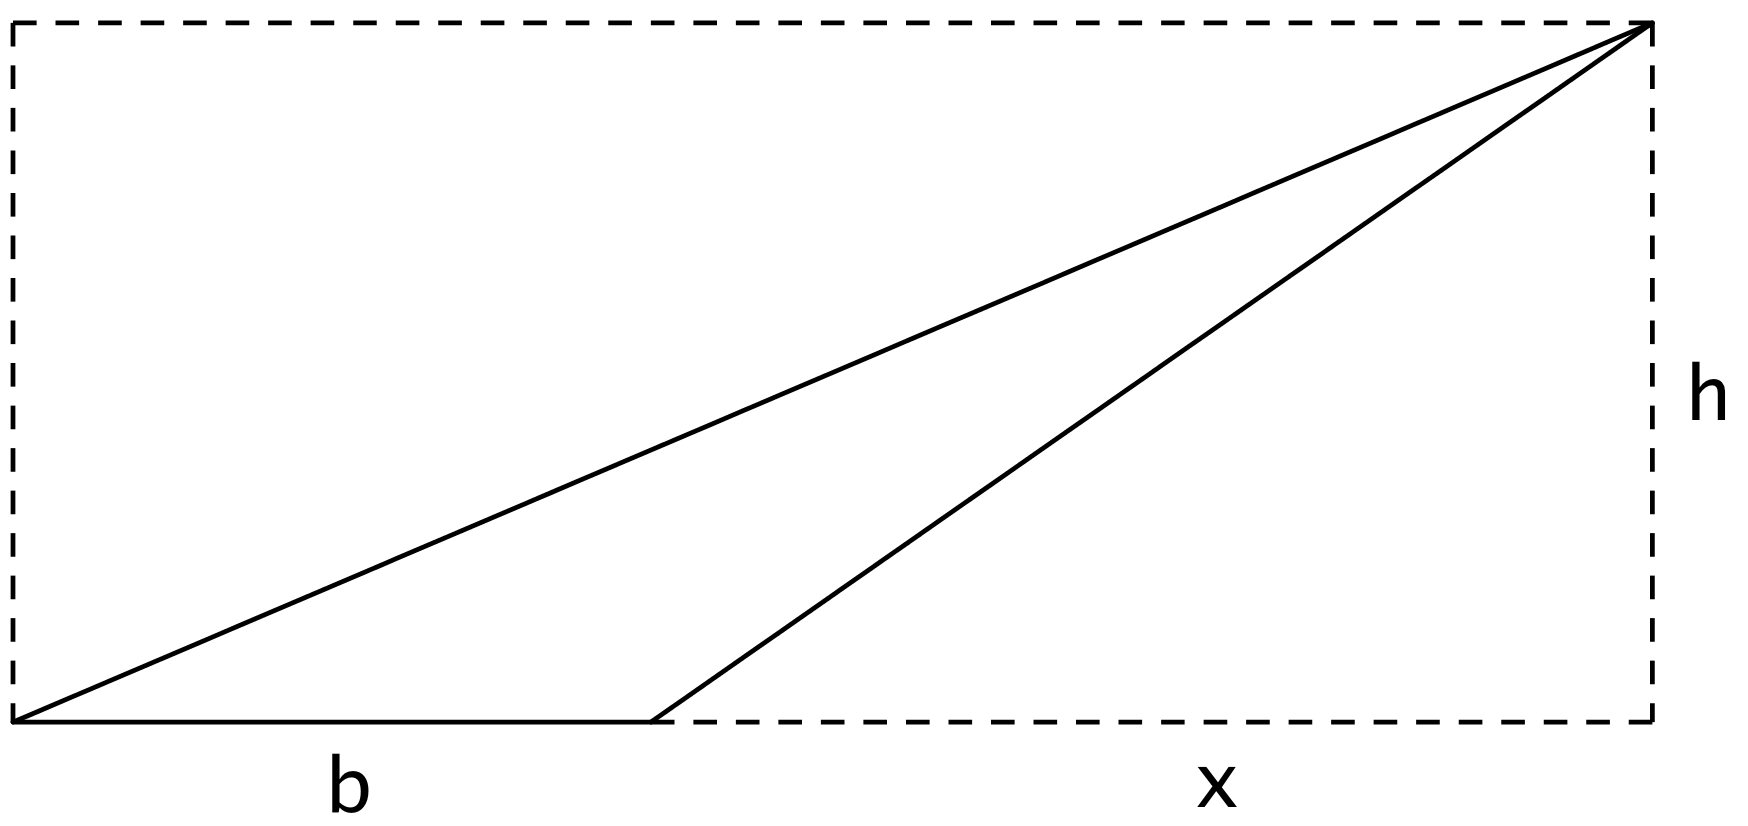
\includegraphics{triangleArea.png}
\end{image}
One way to compute the area of the solid triangle is to (1) compute the area right triangle that is the lower half of the rectangle (with base $b+x$) and then (2) subtract the area of the small right triangle (with base $x$): 
\[
\mathrm{area} =  \answer{\frac{h(b+x)}{2}} - \answer{\frac{hx}{2}}= \frac{hb}{2} + \frac{hx}{2} - \frac{hx}{2} = \answer{\frac{hb}{2}}
\]
\end{hint}
\end{freeResponse}
\end{problem}

%\begin{problem}
%Suppose you know that the area of a \textbf{right} triangle is
%  half the base times the height. Explain how the following picture
%  ``proves'' that the area of any triangle is half the base times the
%  height. Note, this way of thinking is the basis for Cavalieri's
%  Principle.\index{Cavalieri's Principle}
%\begin{image}
%\includegraphics{pbpShearTri.pdf}
%\end{image}
%\item Explain how the following picture ``proves'' that the area of
%  any parallelogram is base times height. Note, this way of thinking
%  is the basis for Cavalieri's Principle.\index{Cavalieri's Principle}
%\begin{image}
%\includegraphics{pbpShearPara.pdf}
%\end{image}
%\begin{freeResponse}
%\end{freeResponse}
%\end{problem}
%
%\begin{problem}
%Explain how to use a picture to ``prove'' that a triangle of a
%  given area could have an arbitrarily large perimeter.
%\begin{freeResponse}
%\end{freeResponse}
%\end{problem}

%\begin{problem}
%Give two explanations of how the following picture ``proves''
%  the Pythagorean Theorem, one using algebra and one without algebra. 
%\begin{image}
%\includegraphics{pbppyth1.pdf}
%\end{image}
%\begin{freeResponse}
%\end{freeResponse}
%\end{problem}
%
%\begin{problem}
%Give two explanations of how the following picture ``proves''
%  the Pythagorean Theorem, one using algebra and one without algebra. 
%\begin{image}
%\includegraphics{pbppyth3.pdf}
%\end{image}
%\begin{freeResponse}
%\end{freeResponse}
%\end{problem}
%
%\begin{problem}
%Explain how the following picture ``proves'' the Pythagorean Theorem.
%\begin{image}
%\includegraphics{pbpdavinci.pdf}
%\end{image}
%Note: This proof is due to Leonardo da Vinci.
%%\item Explain how the following picture ``proves'' the Pythagorean Theorem.
%%\begin{image}
%%\includegraphics{pbppyth2.pdf}
%%\end{image}
%%\item Use the following tessellation to give a dissection proof of the Pythagorean Theorem.
%%\begin{image}
%%\includegraphics{pbppyth2.pdf}
%%\end{image}
%%\item Explain how the following picture ``proves'' the Pythagorean Theorem.
%%\begin{image}
%%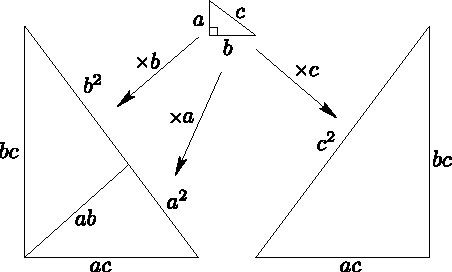
\includegraphics{pbpdilation.pdf}
%%\end{image}
%\begin{freeResponse}
%\end{freeResponse}
%\end{problem}

\begin{problem}
Recall that a trapezoid is a quadrilateral with two parallel sides. Consider the following picture:
\begin{image}
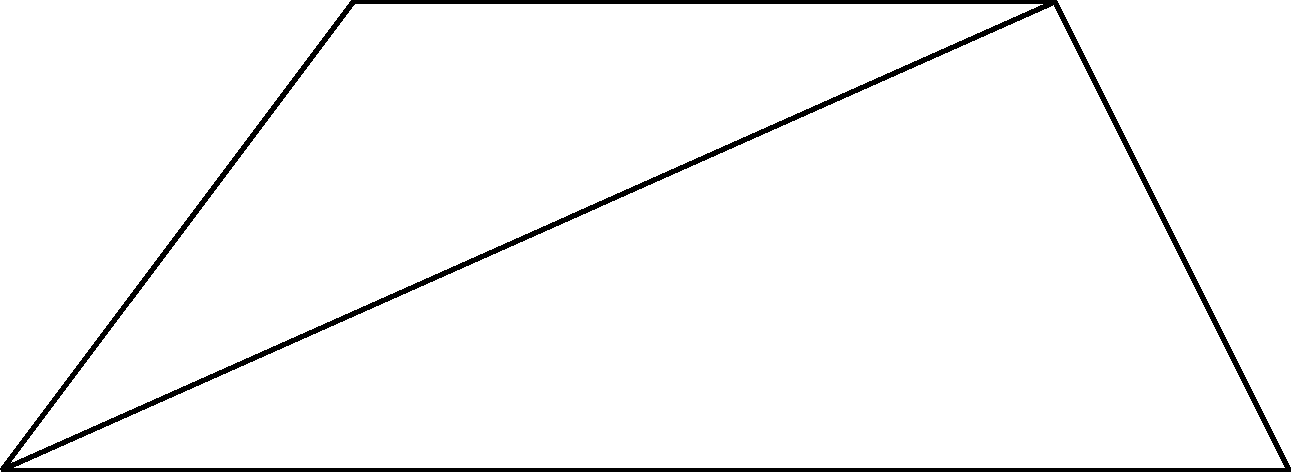
\includegraphics{trap.png}
\end{image}
How does the above picture prove that the area of a trapezoid is
\[
\mathrm{area} = \frac{h(b_1 + b_2)}{2}
\]
where $h$ is the height of the trapezoid and $b_1$, $b_2$, are the lengths of the parallel sides?
\begin{freeResponse}
\begin{hint}
Using the parallel sides as bases, the two triangles have the same height as the trapezoid.  The area of the trapezoid is the sum of the areas of the triangles: 
\[
\mathrm{area} =  \frac{hb_1}{2}+ \frac{hb_2}{2}= \frac{h(b_1 + b_2)}{2}
\]
\end{hint}
\end{freeResponse}
\end{problem}

%\begin{problem}
%Explain how the following picture ``proves'' the Pythagorean Theorem.
%\begin{image}
%\includegraphics{pbptrap.pdf}
%\end{image}
%Note: This proof is due to James A.\ Garfield, the 20th President of the United States.
%\begin{freeResponse}
%\end{freeResponse}
%\end{problem}

\begin{problem}
Look at the previous problem. Can you use a similar idea
  to prove that the area of a parallelogram
\begin{image}
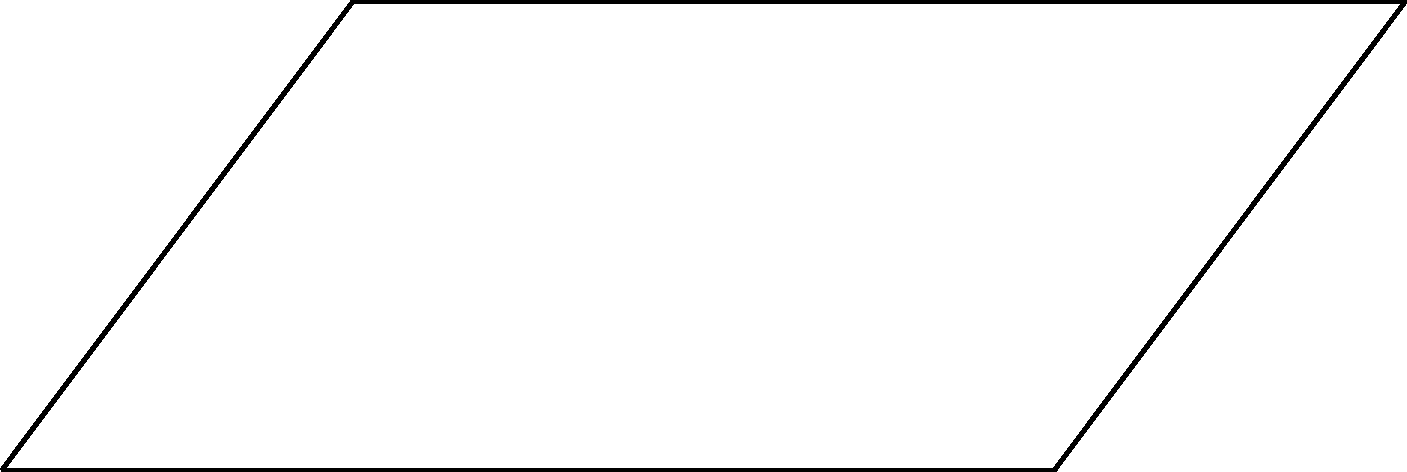
\includegraphics{para.png}
\end{image}
is the length of the base times the height?
\begin{freeResponse}
\begin{hint}
Hint:  Draw a diagonal.  Then there are two triangles with the same base and the same height.  
\end{hint}
\end{freeResponse}
\end{problem}

\begin{problem}
Explain how the following picture ``proves'' that the area of a
  parallelogram is base times height.
\begin{image}
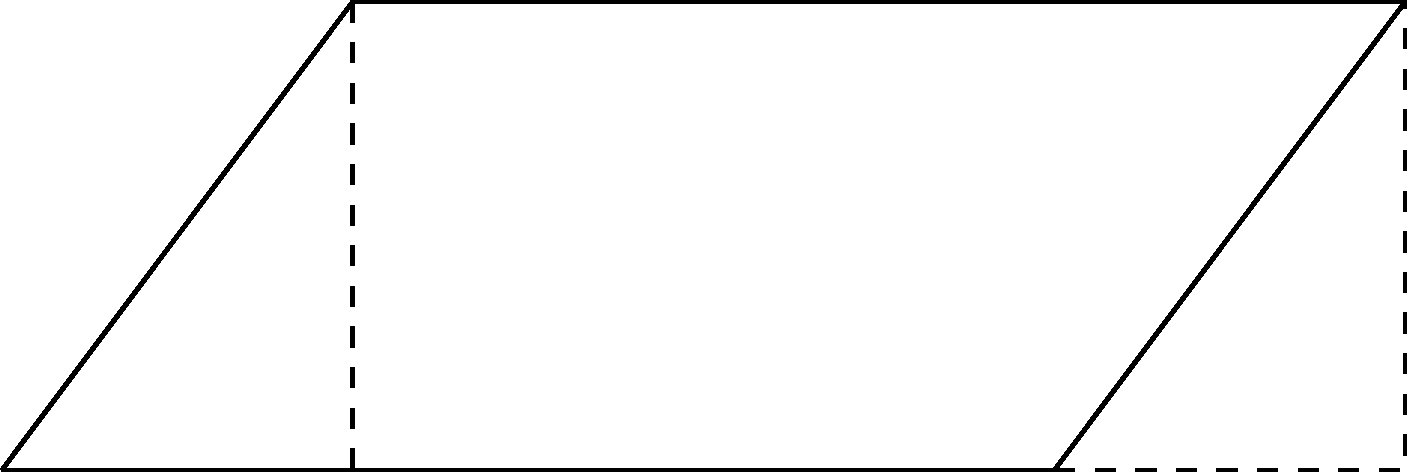
\includegraphics{para3.png}
\end{image}
\begin{freeResponse}
\begin{hint}
Imagine cutting off the triangle on the left and placing it in the (congruent) dotted region on the right.  Then we have a rectangle with the same base and height as the parallelogram.  The cutting and rearranging doesn't change the area of the figure, so the area of the parallelogram is the same as the area of the rectangle, which is $bh$. 
\end{hint}
\end{freeResponse}
\end{problem}

\begin{problem}
Now suppose that a student, say \textit{Geometry Giorgio} attempts to
solve a similar problem. In an attempt to prove the formula for the
area of a parallelogram, \textit{Geometry Giorgio} draws the following
picture:
\begin{image}
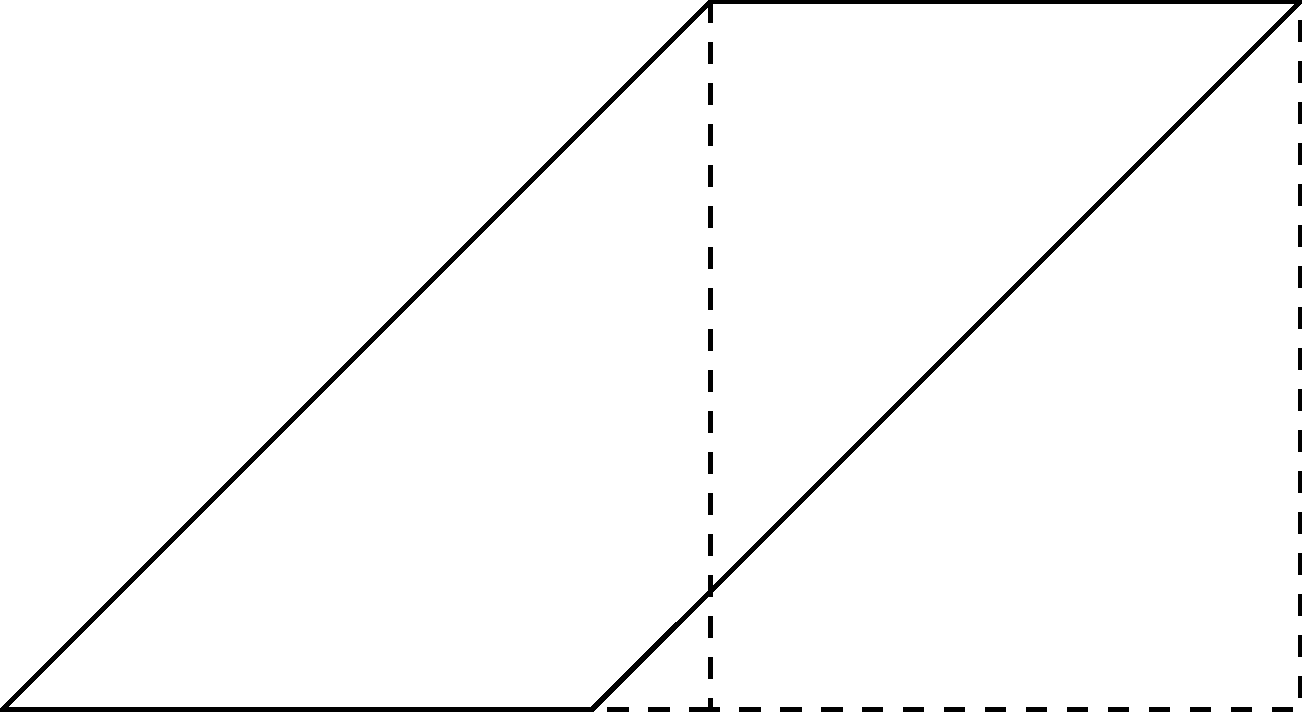
\includegraphics{paragiorgio.png}
\end{image}
At this point \textit{Geometry Giorgio} says that he has proved the
formula for area of a parallelogram. What do you think of his picture?
Give a complete argument based on his picture.
\begin{freeResponse}
\begin{hint}
Hint:  This parallelogram problem is much like Giorgio's triangle problem above.  Use the same idea.  
\end{hint}
\end{freeResponse}
\end{problem}

\end{document}
